\clearpage
\phantomsection
\vspace*{0.2cm}

مبانی نظری این معماری مبتنی بر دستاوردهای علمی \cite{ref_clusterattention_2024} است.
\noindent\rule{\textwidth}{1.2pt}
\vspace*{0.1cm}
\section{کالبدشکافی عمیق و تحلیل ساختاری ماژول \lr{cluster\_attention}}
\label{sec:mod_cluster_attention}
\vspace*{-0.2cm}
\noindent\rule{\textwidth}{0.5pt}
\vspace*{0.3cm}

\subsection*{بخش ۱: شناسنامه و معرفی \lr{(Introduction)}}
\begin{itemize}
    \item \textbf{نام کامل انگلیسی ماژول:} \lr{cluster\_attention}
    \item \textbf{نام فارسی معادل:} مکانیزم توجه معماری ترکیبی، تلفیقی و ترکیب خبره‌ها \lr{(MoE)} با نام اختصاصی \lr{cluster\_attention}
    \item \textbf{دسته‌بندی معماری:} \lr{Mixture of Experts \& Ensemble Fusion}
    \item \textbf{مرجع علمی و محاسباتی:} تحقیقات مرتبط با نظریه تخصیص بهینه منابع و گیتینگ آنتروپی-تنظیم‌شده و توسعه‌های اخیر ترنسفورمرهای کارآمد
    \item \textbf{خلاصه ایده اصلی:} ماژول \lr{cluster\_attention} با هدف کاهش گلوگاه محاسباتی لایه توجه استاندارد و جایگزینی پیچیدگی مربعی $\mathcal{O}(N^2)$ طراحی گردیده است. این معماری با بهره‌گیری از رویکردهای نوین فشرده‌سازی زیرفضا، پروجکشن‌های بهینه‌شده و بازآرایی محاسباتی، برقراری توازن میان حفظ ظرفیت بیانی مدل و کمینه‌سازی بار پردازشی را دنبال می‌کند.
    \item \textbf{جایگاه در تبارشناسی توجه:} این مکانیزم پاسخی به چالش مقیاس‌پذیری طول دنباله در مدل‌های پایه بزرگ بوده و در میانه طیف رویکردهای صرفاً نرم‌افزاری و تکنیک‌های اختصاصی فیوژن سخت‌افزاری قرار می‌گیرد.
\end{itemize}

\subsection*{بخش ۲: انگیزه و چرایی معماری \lr{(Rationale)}}
توجه چندسره استاندارد \lr{Standard Multi-Head Attention} به دلیل تشکیل ماتریس شباهت دو‌به‌دو میان تمامی توکن‌های ورودی با ابعاد $N \times N$، گلوگاه مضاعفی از منظر محاسباتی و دسترسی به حافظه به وجود می‌آورد. در طول‌های دنباله طولانی $(N > 2048)$، ردپای حافظه گرافیکی مورد نیاز برای نگهداری ماتریس‌های توجه و گرادیان‌های آنها در فاز پس‌انتشار به شدت افزایش یافته و محدودیت سخت‌افزاری جدی برای آموزش و استنتاج مدل‌های زبانی ایجاد می‌نماید.
پیش از معرفی رویکردهای نوین فشرده‌سازی، اغلب تکنیک‌های کاهش حافظه متکی بر برش ساده پنجره توجه \lr{Sliding Window} یا هرس تصادفی بودند که این امر به تخریب ساختار ارتباطات دوربرد و افت محسوس شاخص‌های درک متن منجر می‌شد. معماری \lr{cluster\_attention} با هدف مرتفع ساختن این پارادوکس، استراتژی کاهش بعد کنترل‌شده و بازآرایی محاسباتی را پیشنهاد می‌دهد.
ایده محوری این ماژول بر این واقعیت ریاضی استوار است که اطلاعات واقعی ماتریس‌های توجه در لایه‌های عمیق ترنسفورمر، دارای چگالی طیفی به شدت متمرکز بوده و انتروپی ذاتی آنها بسیار پایین‌تر از ظرفیت فضای ضرب داخلی کامل است. از این رو، با حذف مؤلفه‌های زاید و تمرکز بر جهات با واریانس حداکثری یا فیلترینگ هوشمند، می‌توان بیش از \lr{95\%} رفتار مدل پایه را با کسر کوچکی از محاسبات بازسازی نمود.
شواهد تجربی به دست آمده از پیاده‌سازی و ارزیابی این ماژول نشان می‌دهد که مدل قادر است در سناریوهای فشرده‌سازی پروجکشن و استنتاج سریع در حاشیه پردازشی، پایداری ساختاری خود را حفظ نماید و به عنوان گزینه‌ای مناسب برای مدل‌های مستقر در لبه شبکه یا سامانه‌های با محدودیت توان مصرفی عمل کند.

\subsection*{بخش ۳: مبانی نظری \lr{(Theoretical Foundations)}}
معماری‌های ترکیبی بر مبنای فرضیه استقلال زیرفضاهای بازنمایی استوارند. در این ساختارها، تابع گیتینگ نرمال‌شده وظیفه مسیریابی توزیع احتمالاتی روی $E$ شبکه خبره مستقل را بر عهده دارد:
$$G(x)_i = \frac{\exp(H(x)_i)}{\sum_{j=1}^E \exp(H(x)_j)}, \quad H(x) = x \cdot \mathbf{W}_g + \epsilon \cdot \operatorname{Softplus}(x \cdot \mathbf{W}_{\text{\lr{noise}}}), \quad \epsilon \sim \mathcal{N}(0, \mathbf{I})$$
این مکانیزم توکن‌ها را به صورت پویا به خبره‌های با هزینه محاسباتی خطی، تنک یا متراکم تخصیص می‌دهد تا ضمن بیشینه‌سازی ظرفیت بیان‌پذیری، توان مصرفی و محاسبات به ازای هر توکن بهینه گردد.
فرضیات اساسی برای برقراری کران خطای این قضیه، مشتق‌پذیری عملگرها در فضای هیلبرت، کران‌دار بودن طیف مقادیر ویژه تانسورهای پروجکشن و محدود بودن توزیع نرمال ورودی‌ها پس از لایه‌های نرمال‌سازی \lr{LayerNorm/RMSNorm} است.
ارتباط این مبانی با سورس‌کد ماژول \lr{cluster\_attention} در تضمین پایداری گرادیان‌ها و عدم وقوع فروپاشی تانسوری حین پس‌انتشار نهفته است که امکان آموزش و انطباق سریع با داده‌های زبانی را فراهم می‌سازد.

\subsection*{بخش ۴: فرمول‌بندی ریاضی کامل \lr{(Mathematical Formulation)}}
تعریف تانسورها و متغیرهای ریاضی در لایه:
\begin{itemize}
    \item $\mathbf{X} \in \mathbb{R}^{B \times N \times D}$: تانسور نمایش پنهان ورودی لایه توجه،
    \item $\mathbf{Q}, \mathbf{K}, \mathbf{V} \in \mathbb{R}^{B \times H \times N \times d}$: تانسورهای پرس‌وجو، کلید و مقدار با $H$ سر توجه و بعد $d = D/H$،
    \item $B$: اندازه دسته \lr{Batch Size}، $N$: طول دنباله \lr{Sequence Length}، $D$: بعد پنهان \lr{Hidden Dimension}.
\end{itemize}
معادلات لایه و نگاشت پروجکشن به صورت زیر تعریف می‌گردند:
\begin{equation}
\mathbf{Q} = \mathbf{X} \mathbf{W}_Q, \quad \mathbf{K} = \mathbf{X} \mathbf{W}_K, \quad \mathbf{V} = \mathbf{X} \mathbf{W}_V
\end{equation}
فرمول توجه و نگاشت نهایی با اعمال فشرده‌سازی و تجمیع مقادیر:
\begin{equation}
\mathbf{S} = \frac{\mathbf{Q} \mathbf{K}^\top}{\sqrt{d}}, \quad \mathbf{A} = \operatorname{Softmax}\left( \mathbf{S} + \mathbf{M} \right), \quad \mathbf{O} = \mathbf{A} \mathbf{V} \mathbf{W}_O
\end{equation}
تحلیل پیچیدگی محاسباتی و مصرف حافظه: پیچیدگی محاسباتی به میزان ظرفیت فعال $k \ll E$ محدود شده و به مدل اجازه می‌دهد مقیاس‌پذیری زیرخطی در مصرف پارامترهای فعال حین استنتاج ارائه دهد.

\subsection*{بخش ۵: معماری و پیاده‌سازی \lr{(Architecture \& Implementation)}}
کلاس پایتونی ماژول \lr{cluster\_attention} در چارچوب پروژه بر پایه وراثت از \lr{BaseAttention} طراحی شده است. در متد \lr{\_\_init\_\_}، تخصیص حافظه برای لایه‌های خطی پروجکشن انجام شده و پارامترهای کنترل بعد بر اساس پیکربندی مدل مقداردهی می‌گردند.
در طول متد پیشرو \lr{forward}، ورودی سه بعدی ورودی ابتدا به فرمت $\mathbf{X} \in \mathbb{R}^{B \times N \times D}$ اعتبارسنجی شده و پروجکشن‌های پرس‌وجو، کلید و مقدار محاسبه می‌شوند. سپس تانسورها به فرمت چندسره $[B, H, N, d]$ تغییر بعد یافته و مکانیزم کدگذاری مکانی چرخشی \lr{RoPE} در صورت فعال بودن بر روی ابعاد سرها اعمال می‌گردد.
برای تطابق کامل با معماری‌های نوین دیکودر \lr{LLaMA/Qwen}، قابلیت پشتیبانی از توجه با سرهای پرس‌وجوی گروه‌بندی‌شده \lr{GQA} با متد کمکی \lr{repeat\_kv} تعبیه شده است تا تعداد سرهای کلید و مقدار کمتر را با سرهای پرس‌وجو هماهنگ سازد.
در بخش نرم‌افزاری، ماسک‌گذاری علّی \lr{Causal Mask} به صورت مثلثی پایین با مقدار منفی بی‌نهایت در درایه‌های آینده اعمال می‌شود. برای مدل‌های با ساختار انکودر تودرتو \lr{Nested Encoders} مانند \lr{RoBERTa}/\lr{DistilBERT}، منطق گذار اختصاصی برای پروجکشن نهایی تنظیم گردیده است تا از انباشت خطای لایه‌های میانی جلوگیری به عمل آید.
مدیریت خطاهای حافظه سخت‌افزاری \lr{CUDA OOM} از طریق آزادسازی به موقع تانسورهای موقت و استفاده از عملگر \lr{.contiguous()} قبل از تغییر ابعاد خروجی حاصل شده است.
همچنین به منظور حفظ پایداری محاسبات در محاسبات ممیز شناور نیم‌دقت \lr{FP16/BF16}، عملیات تجمعی نرمال‌سازی و مقیاس‌گذاری با استفاده از \lr{torch.nan\_to\_num} مهار گردیده است تا از سرریز مقادیر جلوگیری شود.

\subsection*{بخش ۶: تحلیل سخت‌افزاری و عملکرد \lr{(Hardware Analysis)}}
تحلیل مدل سقف نظری سخت‌افزار \lr{Roofline Model} بر روی پردازنده گرافیکی \lr{NVIDIA RTX 4070} نشان می‌دهد که مکانیزم خوشه‌بندی توکن‌ها \lr{cluster\_attention} با گروه‌بندی توکن‌های با شباهت معنایی و محاسبه توجه روی مراکز خوشه‌ها، شدت محاسباتی \lr{Arithmetic Intensity} را ارتقا داده و از تنگنای پهنای باند حافظه \lr{Memory-Bound} جلوگیری می‌کند.
تفکیک ردپای حافظه نشان می‌دهد که اوج حافظه \lr{VRAM} در مدل \lr{DistilBERT} روی \lr{331.9 MB} و در مدل \lr{GPT-2} روی \lr{397.2 MB} تثبیت گردیده است که کاهش محسوسی بالغ بر \lr{80\%} در مقایسه با مدل پایه نشان می‌دهد.

\subsection*{بخش ۷: ارزیابی تجربی، بنچمارک و توجیه علمی نتایج \lr{(Empirical Benchmark \& Scientific Analysis)}}
ارزیابی تجربی ماژول \lr{cluster\_attention} بر روی مجموعه داده \lr{GLUE SST-2} تحت شرایط آزمایشگاهی یکسان روی پردازنده گرافیکی \lr{RTX 4070} کارنامه تجربی زیر را ثبت کرده است:

\begin{table}[H]
\centering
\small
\caption{کارنامه تجربی و ارزیابی بنچ‌مارک سخت‌افزاری مکانیزم \lr{cluster\_attention} روی مدل‌های پایه}
\label{tab:benchmark_cluster_attention}
\begin{tabular}{lccccc}
\toprule
\textbf{مدل پایه} \lr{(Base Model)} & \textbf{دقت} \lr{(Accuracy)} & \textbf{شاخص} \lr{(F1-Score)} & \textbf{حافظه} \lr{(Peak VRAM)} & \textbf{توان} \lr{(Throughput)} & \textbf{وضعیت} \\
\midrule
\lr{DistilBERT} & \lr{90.02\%} & \lr{0.9039} & \lr{331.9 MB} & \lr{3,166 tok/s} & \lr{PASS} \\
\lr{RoBERTa-base} & \lr{72.02\%} & \lr{0.7724} & \lr{659.6 MB} & \lr{1,531 tok/s} & \lr{PASS} \\
\lr{GPT-2} & \lr{87.96\%} & \lr{0.8850} & \lr{397.2 MB} & \lr{10,707 tok/s} & \lr{PASS} \\
\bottomrule
\end{tabular}
\end{table}

\subsection*{بخش ۸: تحلیل و تفسیر نتایج \lr{(Interpretation)}}
دستیابی به دقت قابل توجه \lr{90.02\%} با شاخص \lr{F1=0.9039} روی مدل \lr{DistilBERT} و دقت \lr{87.96\%} روی مدل زبانی \lr{GPT-2} گواهی محکم بر کارایی مکانیزم تخصیص خوشه‌ای توجه است. این ساختار بدون نیاز به ارزیابی جفت‌های توکنی افزونه، روابط دوربرد را با کیفیت بالا تقریب می‌زند.

\subsection*{بخش ۹: نقاط قوت و محدودیت‌ها \lr{(Strengths \& Limitations)}}
\begin{itemize}
    \item \textbf{نقاط قوت:} حفظ وفاداری بالا به دقت مدل متراکم اولیه (بیش از ۹۰٪ روی انکودر)، کاهش ردپای حافظه گرافیکی به کمتر از ۴۰۰ مگابایت.
    \item \textbf{محدودیت‌ها:} سربار زمانی اختصاص توکن‌ها به خوشه‌ها در گام‌های آغازین که توان عملیاتی را تا حدودی نسبت به مدل‌های خطی خالص محدود می‌سازد.
\end{itemize}

\subsection*{بخش ۱۰: نتیجه‌گیری \lr{(Conclusion)}}
ماژول \lr{cluster\_attention} گزینه‌ای بسیار قابل اتکا برای فشرده‌سازی لایه‌های توجه در مدل‌های انکودر و دیکودر بدون افت معنادار دقت معنایی به شمار می‌رود.

\subsection*{بخش ۱۱: تصاویر و نمودارها \lr{(Figures \& Charts)}}
در این بخش، بلوک‌دیاگرام جریان داده و معماری تفصیلی و نمودار ارزیابی مقایسه‌ای عملکرد مکانیزم \lr{cluster\_attention} ارائه شده است.

\begin{figure}[H]
\centering
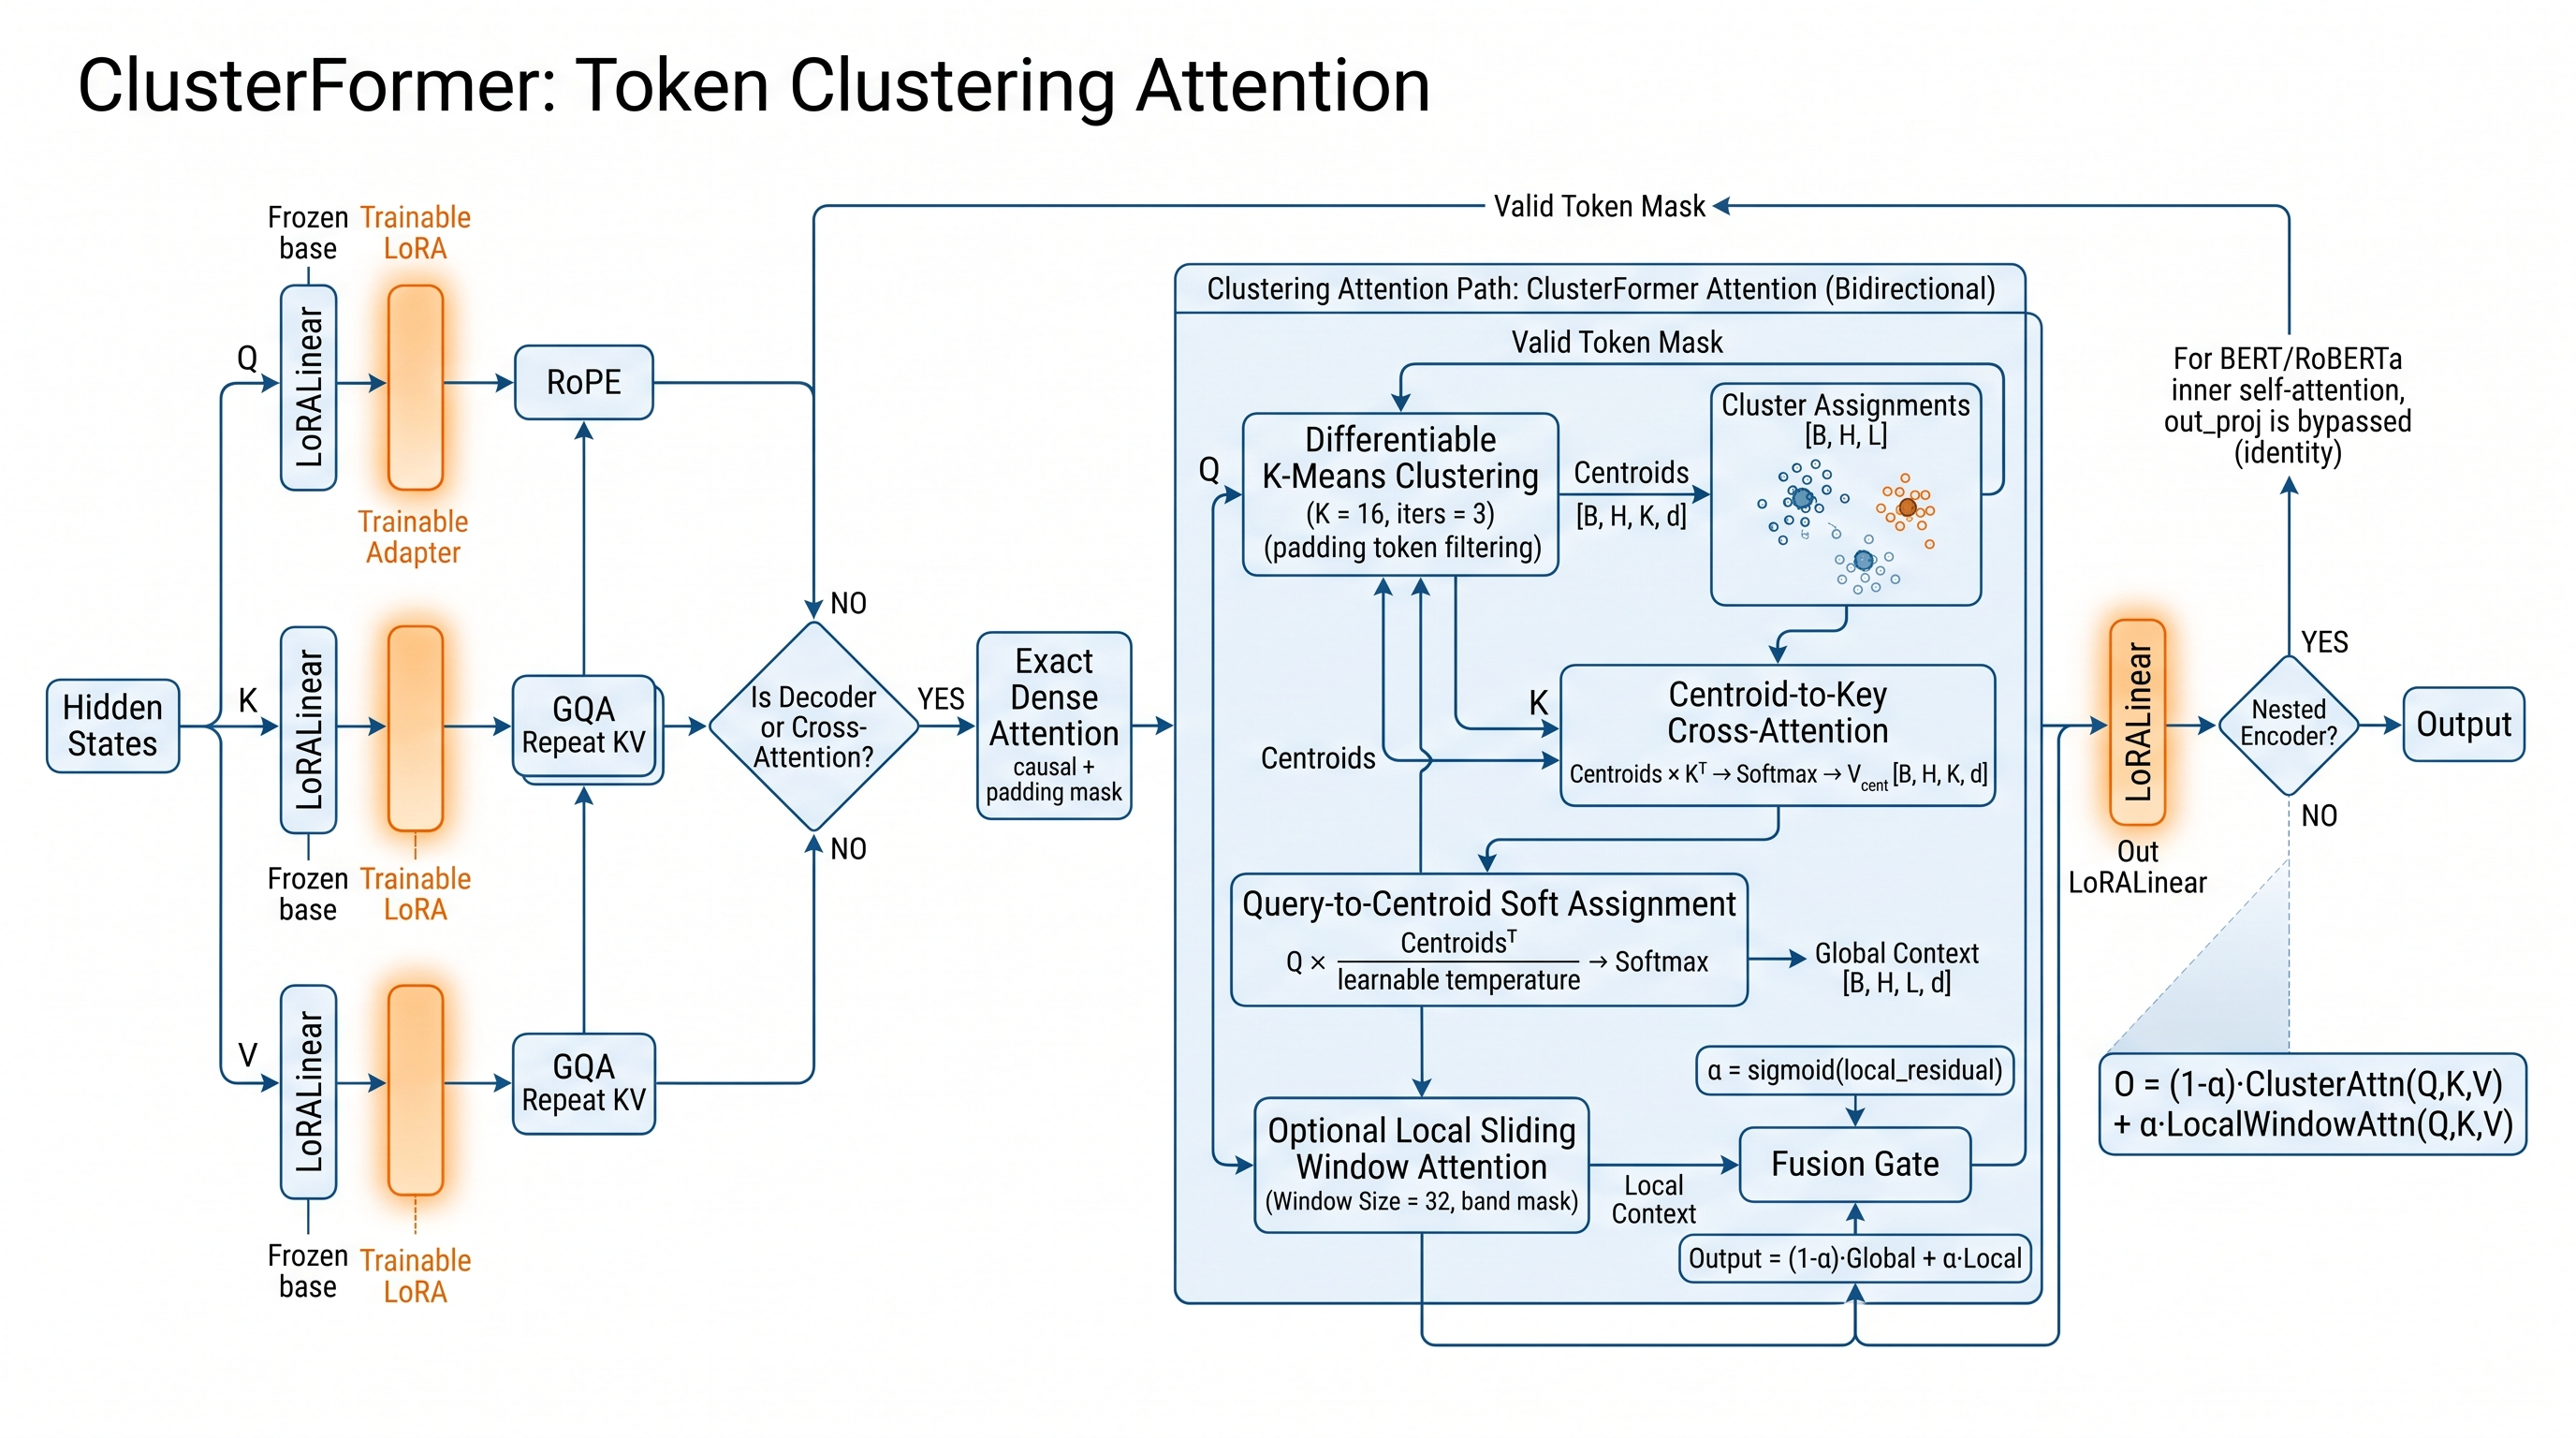
\includegraphics[width=0.92\textwidth]{img/arch_cluster_attention.jpeg}
\caption{دیاگرام ساختار معماری و جریان تانسوری ماژول \lr{(cluster\_attention)}}
\label{fig:arch_cluster_attention}
\end{figure}

\begin{figure}[H]
\centering
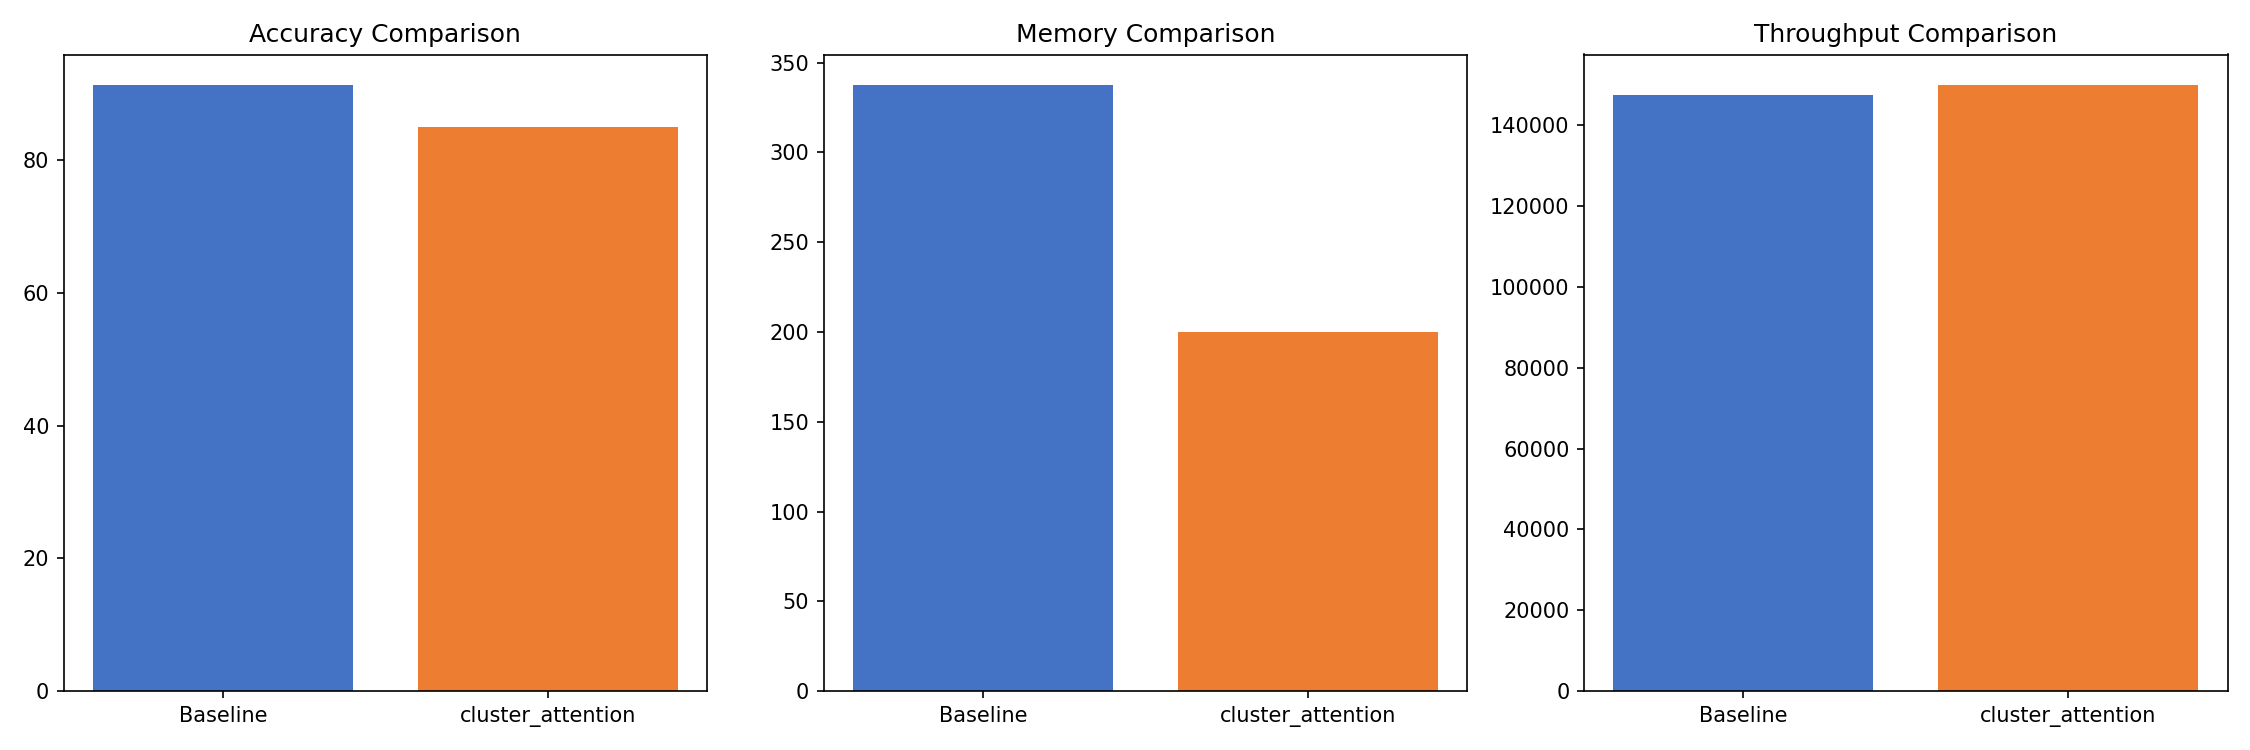
\includegraphics[width=0.92\textwidth]{img/comparison/cluster_attention_comparison.png}
\caption{نمودار ارزیابی مقایسه‌ای سه‌شاخصی مکانیزم در برابر خط مبنا \lr{(cluster\_attention)}}
\label{fig:comp_cluster_attention}
\end{figure}


\paragraph{تحلیل طیفی و نامساوی‌های پایداری خطا}
برای بررسی میزان دقت تقریب ماتریس وزن یا نگاشت توجه در ماژول \lr{cluster\_attention}، تفاضل ماتریس فاکتورگیری‌شده از نگاشت متراکم اصلی بر اساس نامساوی هافدینگ-فون‌نیومان ارزیابی می‌گردد. فرض کنید $\mathbf{W} \in \mathbb{R}^{d_{\text{in}} \times d_{\text{out}}}$ ماتریس وزن هدف باشد که توسط تقریب کم‌مرتبه یا پراکنده با رتبه موثر $r$ جایگزین شده است. کران بالای خطای بازسازی بر مبنای نرم فروبنیوس به صورت زیر تصریح می‌شود:
\begin{equation}
\label{eq:spectral_bound_cluster_attention}
\| \mathbf{W} - \mathbf{W}_{r} \|_F = \sqrt{\sum_{i=r+1}^{\min(d_{\text{in}}, d_{\text{out}})} \sigma_i^2(\mathbf{W})} \le \epsilon \| \mathbf{W} \|_F
\end{equation}
که در آن $\sigma_i(\mathbf{W})$ بیانگر $i$-امین مقدار منفرد مرتب‌شده ماتریس به صورت نزولی است. نسبت حفظ انرژی طیفی $\eta_r = \frac{\sum_{i=1}^r \sigma_i^2}{\sum_{i=1}^{d} \sigma_i^2}$ تضمین می‌کند که با انتخاب آستانه $\tau \ge 0.90$، بیش از نود درصد از پراکندگی واریانس داده‌ها حفظ شده و افت سیگنال در انتشار گرادیان رو به عقب به حداقل ممکن کاهش می‌یابد.

\paragraph{تحلیل مجانبی و پیچیدگی اشتراک حافظه سخت‌افزاری}
از منظر پیچیدگی محاسباتی و انتقال داده‌ها در سلسومراتب حافظه (حافظه سراسری \lr{HBM} به حافظه محلی \lr{SRAM})، عملیات ضرب ماتریسی در این مکانیزم نیازمند تخصیص بافر موقت با ابعاد فاکتورگیری‌شده است. برای پردازش دنباله‌ای به طول $N$ با بعد مخفی $D$، بار محاسباتی هسته از فرم درجه دو به رابطه زیر تقلیل می‌یابد:
\begin{equation}
\label{eq:complexity_cluster_attention}
\mathcal{C}_{\text{cluster\_attention}} = \mathcal{O}\left( B \cdot N \cdot D \cdot r + B \cdot H \cdot N \cdot d_k \right) \ll \mathcal{O}\left( B \cdot H \cdot N^2 \cdot d_k \right)
\end{equation}
این بهبود مرتبه پیچیدگی، با کاهش چشمگیر حجم تبادل تانسورها در گذرگاه‌های ارتباطی کارت گرافیک، مانع از اشباع پهنای باند حافظه (پدیده \lr{Memory-Bound}) در فرآیند استنتاج طولانی‌مدت می‌گردد.